\chapter{Strutture dati e algoritmi utilizzati}
\label{sec:strutture dati e algoritmi utilizzati}

\begin{table}[]
    \centering
    \setcellgapes{3pt}
    \makegapedcells
    \begin{tabular}{|c|c|c|}
    \hline
    \textbf{Nome del package} & \textbf{Numero di classi} & \textbf{Descrizione}\\ \hline
    DB & 3 & Collegamento al database\\ \hline
    Model & 14 & Algoritmi\\ \hline
    SimulazioneF1 & 5 & Controller interfaccia grafica\\ \hline
    \end{tabular}
    \caption{schema dei package}
    \label{tab:schema dei package}
\end{table}
% use [] to set name for ToC
\section[Struttura del progetto]{Struttura del progetto} % ok with fontsize=12pt
L'applicazione, scritta in linguaggio Java, segue il pattern  pattern MVC(Model View Controller), quindi dividendo la struttura software in 3 parti principali: model, view e controller. Inoltre l'applicazione sfrutta il pattern DAO (Database Access Object), che permette di accedere ai dati sul database, basandosi sugli input dell'utente (ad esempio il numero di gare) e ricavando informazioni poi processate dal Model.\\
Il progetto dell'applicazione è disponibile nel repository Github al seguente link: \href{https://github.com/TdP-prove-finali/CiuffredaEnrico}{https://github.com/TdP-prove-finali/CiuffredaEnrico}.\\
Il progetto si compone di 3 package:
\begin{itemize}

    \item\textbf{ DB}: contiene tutte le classi utili a: collegarsi al database ed estrarne i dati seguendo il pattern DAO;
    \item \textbf{Model}: contiene tutte le classi utilizzati per memorizzare i dati, tutte le classi necessarie per la memorizzazione dei dati, le classi utilizzate per stampare dei dati e le classi utilizzate per la generazione degli eventi gara e qualifica e quindi per la loro simulazione;
    \item \textbf{SimulazioneF1}: contiene tutte le classi per gestire l'interfaccia grafica dell'applicazione. Al suo interno è disponibile una classe \textit{Controller} per ognuna delle due scene, la prima che permette al pilota di impostare alcuni parametri nella simulazione e la seconda utilizzata per stampare a schermo i risultati ottenuti dalla simulazione. La classe \textit{CambiaScena} è invece utlizzata per passare dalla prima scena alla seconda e viceversa.
\end{itemize}
\section[Software utilizzati]{Software utilizzati} % ok with fontsize=12pt
L'applicazione è stata realizzata tramite l'IDE Ecplise. Per la realizzazione di parte dell'interfaccia grafica è stato utilizzato il software SceneBuilder.\\
Il DBMS utilizzato è MariaDB con interfaccia grafica HeidiSQL.
\begin{figure}[h]
\centering
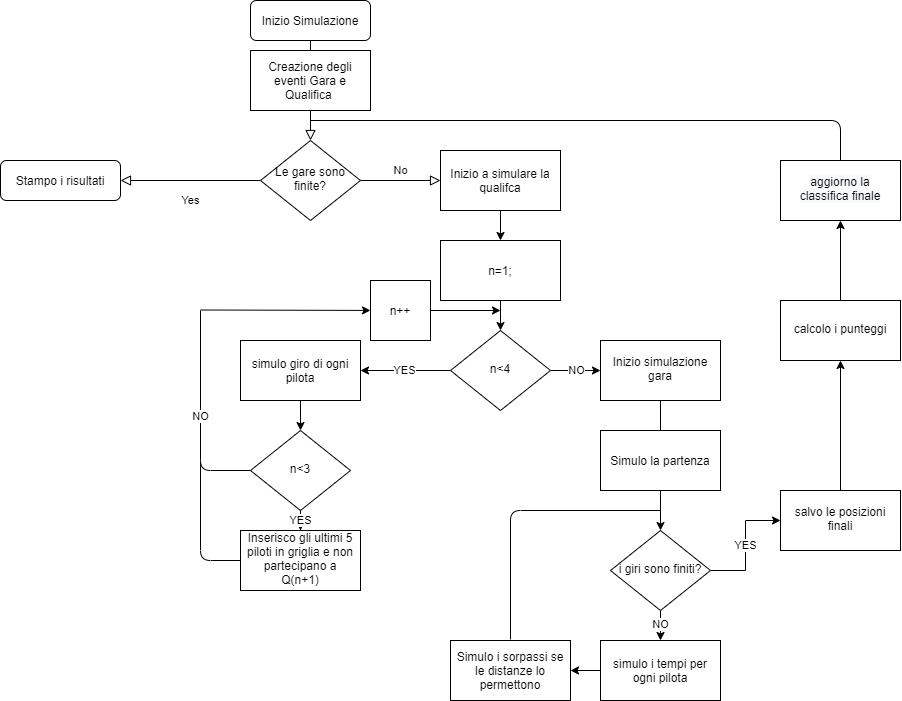
\includegraphics[width=1\linewidth]{images/Flowchart simulazione.png}
\caption{Flowchart simulazione}
\label{fig:Flowchart simulazione}
\end{figure}

\section[Algoritmi]{Algoritmi} % ok with fontsize=12pt
L'applicazione presenta alcuni algoritmi fondamentali.
\subsection{Algoritmo di modifica dati in base a parametri scelti dall'utente}
Lo scopo di questo algoritmo, contenuto nella classe \textit{Model}, è quello di poter permettere all'utente di influenzare la simulazione attraverso 3 procedure: 
\begin{itemize}
\item Sostituzione di un pilota presente in lista con un pilota con dati introdotti dall'utente;
\item Scambio di scuderia tra due piloti. Lo scambio prevede che i tempi dei piloti siano diminuiti o aumentati in base alla differenza di punteggio assegnato alle due diverse macchine;
\item Miglioramento di una scuderia attraverso l'investimento di un numero, inserito dall'utente, di milioni di euro. L'investimento fa sì che i tempi dei giri di gara e qualifica dei due piloti della scuderia vengano diminuiti in base al miglioramento apportato alla macchina utilizzando questi nuovi fondi.
\end{itemize}
\subsection{Algoritmo di generazione eventi}
Lo scopo di questo algoritmo, contenuto nella classe \textit{Simulatore}, è quello di generare gli eventi su cui effettuare la simulazione. Come possiamo notare dalla classe \textit{Evento}, abbiamo due tipi di eventi che possono essere creati: evento QUALIFICA ed evento GARA; questi eventi vengono generati insieme poichè ad ogni gara deve corrispondere una ed una sola qualifica ed ad ogni qualifica deve corrispondere una ed una sola gara. Questo algoritmo utilizza i dati proveniente dal database per scegliere quali sono i circuiti in cui i piloti dovranno gareggiare.
\subsection{Algoritmo di simulazione della qualifica}
Lo scopo di questo algoritmo, contenuto nella classe \textit{SimulatoreQualifica}, è quello di riuscire a simulare l'intera qualifica e quindi di poter generare una griglia di partenza per la gara del giorno successivo. L'algoritmo può essere diviso in diverse parti:
\begin{itemize}

    \item \textbf{Simulazione del giro}: in base ai risultati ottenuti da un pilota nelle qualifiche degli anni precedenti viene stimato un tempo di percorrenza del giro. Questo tempo viene poi diminuito o aumentato in base ad una variabile casuale (ogni valore viene aumentato in percentuale se durante la qualifica piove);
    \item \textbf{Calcolo del tempo impiegato per un giro}: nel caso in cui il pilota, del quale si vuole calcolare il tempo di percorrenza del giro, non abbia mai corso su quel circuito allora il tempo del giro viene calcolato attraverso un algoritmo basato sulla differenza di abilità tra il pilota e un altro pilota estratto da quelli presenti in lista e sulla differenza del punteggio assegnato alla macchina del pilota e dello stesso pilota scelto come confronto. Questo tempo viene poi diminuito o aumentato in base ad una variabile casuale (ogni valore viene aumentato in percentuale se durante la qualifica piove);
    \item \textbf{Sostituzione piloti infortunati e incidenti}: Ad ogni giro compiuto da un pilota è presente una probabilità che esso faccia un incidente. L'incidente può essere di 3 entità: 
    \begin{enumerate}
    \item il pilota rimane illeso e può partecipare alla gara ma parte nell'ultima posizione disponibile. Nel caso l'incidente avvenga in Q1 la posizione è uguale all'ultimo posto, in Q2 equivale al quindicesimo posto e in Q3 equivale al decimo posto;
    \item il pilota dovrà saltare la gara del giorno dopo;
    \item il pilota dovrà saltare la gara del giorno dopo e un'ulteriore gara.
    \end{enumerate}
    Nei casi in cui un pilota è infortunato viene sostiuito da un altro pilota che potrà ottenere punti per la scuderia e punti per sè stesso ma non per il pilota che viene sostiuito.
    \item \textbf{Aggiornamento griglia di partenza}: Il sistema knock-out, utilizzato in F1, prevede 3 step. Al primo step partecipano tutti i piloti. Alla fine dei primi due step vengono eliminati 5 piloti e le loro posizioni in griglia di partenza vengono calcolate in base ai loro tempi. Nell'ultimo step vengono poi assegnati le prime dieci posizione in base allo stesso criterio.
\end{itemize}
\subsection{Algoritmo di simulazione della gara}
Lo scopo di questo algoritmo, contenuto nella classe \textit{SimulatoreGara}, è quello di riuscire a simulare l'intera gara e quindi di poter assegnare i punti in base alla posizione finale del pilota. L'algoritmo può essere diviso in diverse parti:
\begin{itemize}

    \item \textbf{Simulazione del giro}: in base ai risultati ottenuti da un pilota nelle gare degli anni precedenti sullo stesso circuito viene stimato un tempo di percorrenza del giro. I giri sono suddivisi in gruppi di cinque poichè in questo modo è possibile considerare l'usura delle gomme e attenuare l'effetto di un pitstop sul tempo di percorrenza di un giro. Questo tempo viene poi diminuito o aumentato in base ad una variabile casuale (ogni valore viene aumentato in percentuale se durante la qualifica piove);
    \item \textbf{Calcolo del tempo impiegato per un giro}: nel caso in cui il pilota, del quale si vuole calcolare il tempo di percorrenza del giro, non abbia mai corso su quel circuito allora il tempo del giro viene calcolato attraverso un algoritmo basato sulla differenza di abilità tra il pilota e un altro pilota estratto da quelli presenti in lista e sulla differenza del punteggio assegnato alla macchina del pilota e dello stesso pilota scelto come confronto. Questo tempo viene poi diminuito o aumentato in base ad una variabile casuale (ogni valore viene aumentato in percentuale se durante la qualifica piove);
    \item \textbf{Sostituzione piloti infortunati e incidenti}: Ad ogni giro compiuto da un pilota è presente una probabilità che esso faccia un incidente. L'incidente può essere di 3 entità: 
    \begin{enumerate}
    \item il pilota rimane illeso ma il tempo di ogni giro viene aggravato da una penalità che ne aumenta il tempo di percorrenza di un giro di un quarto;
    \item il pilota non terminerà la gara in corso;
    \item il pilota non terminerà la gara in corso e non prenderà parte alla prossima gara.
    \end{enumerate}
    Nei casi in cui un pilota è infortunato viene sostiuito da un altro pilota che potrà ottenere punti per la scuderia e punti per sè stesso ma non per il pilota che viene sostiuito.
\end{itemize}
